% !TEX TS-program = xelatex
% !TEX encoding = UTF-8 Unicode
% ═══════════════════════════════════════════════════════════════════════════════
% التقرير الأكاديمي والتطبيقي الشامل لمشروع بناء مترجم لغة البرمجة العربية ومحرر الأكواد
% مقرر: بناء المترجمات وتصميم لغات البرمجة (CS 351)
% جامعة إب - كلية الحاسوب وتكنولوجيا المعلومات - قسم تقنية المعلومات / علوم الحاسوب
% إشراف أستاذ المقرر: د. خالد الكحصة | إشراف مدرس العملي: أ/ عقيل الشرفي
% العام الجامعي: 2025 / 2026 م (1446 / 1447 هـ) - الفصل الدراسي الأول
% التوثيق وفق معايير الجمعية الأمريكية لعلم النفس (APA 7th Edition)
% ═══════════════════════════════════════════════════════════════════════════════

\documentclass[11pt,a4paper,oneside]{report}

% ── حزم الخطوط واللغة العربية والإعدادات الطباعية ─────────────────────────────────────
\usepackage{geometry}
\geometry{a4paper, left=2.0cm, right=2.0cm, top=2.5cm, bottom=2.5cm}

\usepackage{fontspec}
\usepackage{polyglossia}
\setmainlanguage[numerals=maghrib]{arabic}
\setotherlanguage{english}

% تعيين الخطوط للنصوص العربية والإنجليزية
\newfontfamily\arabicfont[Script=Arabic, Scale=1.1]{Traditional Arabic}
\newfontfamily\arabicfonttt[Script=Arabic, Scale=0.95]{Segoe UI}
\setmainfont{Times New Roman}
\setmonofont{Consolas}

\usepackage{amsmath,amssymb}
\usepackage{graphicx}
\usepackage{booktabs}
\usepackage{array}
\usepackage{longtable}
\usepackage{tabularx}
\usepackage{xcolor}
\usepackage{fancyhdr}
\usepackage{titlesec}
\usepackage{listings}
\usepackage{tcolorbox}
\tcbuselibrary{skins,breakable}
\usepackage{hyperref}

% ── لوحة الألوان الأكاديمية المعتمدة ──────────────────────────────────────────
\definecolor{NavyBlue}{HTML}{0D2137}
\definecolor{RoyalBlue}{HTML}{1A4D8F}
\definecolor{AccentCyan}{HTML}{2E86AB}
\definecolor{GoldYellow}{HTML}{C9943A}
\definecolor{BgLight}{HTML}{F8FAFC}
\definecolor{BorderGray}{HTML}{CBD5E1}
\definecolor{TextDark}{HTML}{1E293B}

% ── إعدادات الروابط التشعبية ────────────────────────────────────────────────
\hypersetup{
    colorlinks=true,
    linkcolor=RoyalBlue,
    citecolor=NavyBlue,
    urlcolor=AccentCyan,
    pdfauthor={مجموعة مشروع المترجمات - جامعة إب},
    pdftitle={تقرير مشروع مترجم لغة البرمجة العربية ومحرر الأكواد - C++20},
    pdfsubject={بناء المترجمات وتصميم لغات البرمجة (CS 351)}
}

% ── إعدادات الترويسة والتذييل ────────────────────────────────────────────────
\pagestyle{fancy}
\fancyhf{}
\fancyhead[R]{\small\textcolor{NavyBlue}{\arabicfont مترجم لغة البرمجة العربية (C++20) وبيئة المحرر المستقلة}}
\fancyhead[L]{\small\textcolor{NavyBlue}{CS 351 | Ibb University}}
\fancyfoot[R]{\small\textcolor{gray}{\arabicfont جامعة إب - كلية الحاسوب وتكنولوجيا المعلومات}}
\fancyfoot[L]{\small\textcolor{gray}{Page \thepage}}
\renewcommand{\headrulewidth}{0.8pt}
\renewcommand{\footrulewidth}{0.5pt}

% ── تنسيق عناوين الفصول والأقسام ─────────────────────────────────────────────
\titleformat{\chapter}[display]
  {\normalfont\huge\bfseries\color{NavyBlue}\arabicfont}
  {\filleft\Large\textcolor{GoldYellow}{\chaptertitlename\ \thechapter}}
  {1ex}
  {\titlerule[1.5pt]\vspace{1ex}\filleft}
\titleformat{\section}
  {\normalfont\Large\bfseries\color{RoyalBlue}\arabicfont}
  {\thesection}{1em}{}
\titleformat{\subsection}
  {\normalfont\large\bfseries\color{NavyBlue}\arabicfont}
  {\thesubsection}{1em}{}

% ── تنسيق بيئات الأكواد البرمجية ─────────────────────────────────────────────
\lstset{
    basicstyle=\ttfamily\small\color{TextDark},
    backgroundcolor=\color{BgLight},
    frame=single,
    rulecolor=\color{BorderGray},
    breaklines=true,
    breakatwhitespace=true,
    tabsize=4,
    showstringspaces=false,
    keywordstyle=\color{RoyalBlue}\bfseries,
    commentstyle=\color{gray}\itshape,
    stringstyle=\color{GoldYellow}
}

% ═══════════════════════════════════════════════════════════════════════════════
% بداية وثيقة التقرير الأكاديمي
% ═══════════════════════════════════════════════════════════════════════════════
\begin{document}

% ── صفحة الغلاف الأكاديمي الرسمي (Cover Page) ──────────────────────────────────
\begin{titlepage}
\begin{center}
    {\Large\bfseries\color{NavyBlue}\arabicfont جامعة إب -- Ibb University}\\[0.3cm]
    {\large\color{RoyalBlue}\arabicfont كلية الحاسوب وتكنولوجيا المعلومات -- قسم تقنية المعلومات / علوم الحاسوب}\\[0.5cm]
    \textcolor{GoldYellow}{\rule{\textwidth}{2pt}}\\[1.2cm]

    {\large\bfseries\color{GoldYellow}\arabicfont التقرير الأكاديمي والتطبيقي الشامل لمشروع التخرج والمقرر}\\[0.4cm]
    {\huge\bfseries\color{NavyBlue}\arabicfont مشروع بناء مترجم لغة البرمجة العربية ومحرر الأكواد المستقل}\\[0.3cm]
    {\Large\bfseries\color{AccentCyan} Arabic Language Compiler (Modern C++20) \& Standalone IDE (.NET 9)}\\[1.5cm]

    \begin{tcolorbox}[colback=BgLight,colframe=RoyalBlue,arc=4mm,width=0.92\textwidth]
    \centering
    \begin{tabular}{r p{9.5cm}}
        \textbf{\color{NavyBlue}\arabicfont اسم المقرر:} & \arabicfont بناء المترجمات وتصميم لغات البرمجة (CS 351) \\[0.25cm]
        \textbf{\color{NavyBlue}\arabicfont إشراف أستاذ المقرر:} & \arabicfont الدكتور القدير / خالد الكحصة \\[0.25cm]
        \textbf{\color{NavyBlue}\arabicfont إشراف مدرس العملي:} & \arabicfont الأستاذ المهندس / عقيل الشرفي \\[0.35cm]
        \textbf{\color{NavyBlue}\arabicfont أعضاء المجموعة (5 طلاب):} & 
        \arabicfont 1. يعقوب خالد المهاجري \\
        & \arabicfont 2. سليمان صالح العربي \\
        & \arabicfont 3. مالك عادل جبران \\
        & \arabicfont 4. [اسم عضو المجموعة الرابع] \\
        & \arabicfont 5. [اسم عضو المجموعة الخامس] \\[0.35cm]
        \textbf{\color{NavyBlue}\arabicfont الفصل الدراسي:} & \arabicfont الفصل الدراسي الأول \\[0.25cm]
        \textbf{\color{NavyBlue}\arabicfont العام الجامعي:} & \arabicfont 2025 / 2026 م (1446 / 1447 هـ) \\
    \end{tabular}
    \end{tcolorbox}

    \vfill
    \textcolor{GoldYellow}{\rule{\textwidth}{1.5pt}}\\[0.2cm]
    {\small\color{gray}\arabicfont توثيق أكاديمي رسمي خاضع لمعايير الجمعية الأمريكية لعلم النفس (APA 7th Edition) ومواصفات قسم علوم الحاسوب}
\end{center}
\end{titlepage}

% ── فهرس المحتويات والجداول والأشكال ─────────────────────────────────────────
\tableofcontents
\newpage

% ═══════════════════════════════════════════════════════════════════════════════
% الفصل الأول: وصف المشروع وهندسته المعمارية
% ═══════════════════════════════════════════════════════════════════════════════
\chapter{وصف فكرة المشروع وهندسته المعمارية}

\section{فكرة المشروع وأهدافه التعليمية}
يمثل هذا المشروع تطبيقا عمليا وهندسيا شاملا لمفاهيم بناء المترجمات (Compiler Construction) وبيئات التطوير المتكاملة (IDEs). يهدف المشروع إلى تصميم وبناء نظام برمجي مستقل قادر على ترجمة برامج مكتوبة بلغة برمجة عربية فصحى عالية المستوى وتنفيذها محليا بدقة وأمان.

تم تصميم النظام برمجيا ومعماريا على هيئة \textbf{برنامجين تنفيذيين مستقلين تماما (Two Independent Executables)}:
\begin{enumerate}
    \item \textbf{المترجم المستقل (\texttt{CompilerProject\_CPP.exe}):} مطور كليا بلغة \textbf{Modern C++20} بدون أي مولدات خارجية (Handwritten Multi-Phase Compiler)، ويطبق المراحل الست الكلاسيكية للترجمة.
    \item \textbf{محرر لغة البرمجة العربية (\texttt{LanguageEditor.exe}):} بيئة تطوير تفاعلية ذات واجهة رسومية أصيلة تدعم اتجاه الكتابة من اليمين إلى اليسار (RTL)، مبنية باستخدام C\# 13 و .NET 9.
\end{enumerate}

\section{الفصل المعماري وآلية الاتصال بين المحرر والمترجم (IPC Architecture)}
التزاما بالتعليمات الأكاديمية الصارمة للمشروع، تم فصل المحرر عن المترجم فصلا تاما في مسارين تشغيليين منفصلين:
\begin{itemize}
    \item يقوم المحرر الرسومي بحفظ الكود في ملف مصدري مؤقت (\texttt{source.arb}) بترميز UTF-8.
    \item يستدعي المحرر عملية المترجم عبر الأنابيب البرمجية:
    \texttt{CompilerProject\_CPP.exe "source.arb" --json}.
    \item يمرر المحرر مدخلات المستخدم لتعليمة \texttt{اقرا} عبر مجرى الدخل القياسي (\texttt{StandardInput}) لعملية المترجم بدون تعليق أو Deadlock.
    \item ينفذ المترجم كافة المراحل الست ويطبع كائن JSON متكامل على مجرى الإخراج القياسي (\texttt{StandardOutput}).
    \item يستلم المحرر مخرجات JSON ويفككها لحظيا لتغذية تبويبات العرض الثمانية.
\end{itemize}

% ═══════════════════════════════════════════════════════════════════════════════
% الفصل الثاني: لغات البرمجة والأدوات والمكتبات
% ═════════════════════════════════════════════════════════════════════════
\chapter{لغات البرمجة والأدوات والمكتبات المستخدمة}

\section{لغات البرمجة المعتمدة وإصداراتها}
\begin{itemize}
    \item \textbf{Modern C++ (ISO/IEC 14882:2020 -- C++20):} استخدمت لبناء نواة المترجم المستقل بالكامل (\texttt{CompilerProject\_CPP.exe}). تم تجميع الكود عبر مترجم \texttt{MSVC 19.4x} مع التحسين الأقصى \texttt{/O2} و \texttt{/std:c++20}.
    \item \textbf{C\# (Version 13.0 / .NET 9.0 SDK):} استخدمت لبناء بيئة التطوير الرسومية والمحرر التفاعلي (\texttt{LanguageEditor.exe}).
\end{itemize}

\section{جدول الأدوات والمكتبات الجاهزة وتوصيفها الأكاديمي}
\begin{longtable}{|p{4.2cm}|p{2.2cm}|p{6.8cm}|p{3.2cm}|}
\hline
\rowcolor{NavyBlue}\color{white}\textbf{\arabicfont اسم الأداة / المكتبة} & \rowcolor{NavyBlue}\color{white}\textbf{\arabicfont الإصدار} & \rowcolor{NavyBlue}\color{white}\textbf{\arabicfont الغرض من الاستخدام} & \rowcolor{NavyBlue}\color{white}\textbf{\arabicfont الجزء المستخدم فيه} \\
\hline
\endhead
C++ Standard Library (STL) & C++20 & إدارة الذاكرة الآمنة عبر المؤشرات الذكية (\texttt{shared\_ptr}) وهياكل البيانات الديناميكية وجداول التجزئة السريعة $O(1)$. & كافة مراحل مترجم C++ \\
\hline
Microsoft Visual C++ (MSVC) & v19.4x (2022) & تجميع وترجمة كود المترجم إلى ملف تنفيذي أصلي فائق السرعة والأداء. & نواة المترجم المستقل \\
\hline
Windows Console Win32 API & Win32 API & ضبط وتوحيد ترميز سطر الأوامر على UTF-8 وقراءة مجرى Stdin للأنابيب بدون حجب الخيوط. & ملف \texttt{main.cpp} في C++ \\
\hline
Windows Forms (.NET 9) & v9.0 Core & بناء الواجهة الرسومية التفاعلية للمحرر ودعم اتجاه النصوص العربي RTL وتبويبات العرض. & \texttt{LanguageEditor (MainForm)} \\
\hline
System.Diagnostics.Process & .NET 9.0 & استدعاء عملية المترجم في الخلفية وتمرير وسائط JSON ومتابعة قنوات الإدخال والإخراج. & ملف \texttt{MainForm.cs} \\
\hline
Inno Setup Compiler & v6.3.3 & حزم المترجم والمحرر في حزمة إعداد وتثبيت تنفيذي مستقل وشامل (\texttt{PREXE-GXX.exe}). & حزمة التثبيت النهائي \\
\hline
\end{longtable}

% ═══════════════════════════════════════════════════════════════════════════════
% الفصل الثالث: الشرح البرمجي المفصل لمترجم C++ وفق العناصر التسعة
% ═════════════════════════════════════════════════════════════════════════
\chapter{الشرح التفصيلي لأكواد مترجم C++ وفق العناصر التحليلية التسعة}

وفقا للتعليمات الرسمية المحددة للتقرير، يتم شرح كل جزء برمجي في مترجم C++ وبيئة المحرر وفق \textbf{العناصر التحليلية التسعة الإلزامية}:
(1) وظيفة الجزء، (2) المدخلات، (3) المخرجات، (4) المتغيرات، (5) هياكل البيانات، (6) الدوال والإجراءات، (7) المكتبات، (8) الملفات المرتبطة، (9) كيفية الارتباط بباقي أجزاء المشروع.

\section{نماذج البيانات وعقد شجرة الإعراب (\texttt{Token.h}, \texttt{Node.h}, \texttt{CompilationResult.h})}
\begin{tcolorbox}[colback=BgLight,colframe=BorderGray,title={\small\arabicfont مقطع من كود نماذج البيانات C++20}]
\begin{lstlisting}[language=C++]
struct Token {
    TokenType Type;
    std::string Value;
    int Line = 0;
    Token(TokenType t, std::string v, int l) : Type(t), Value(v), Line(l) {}
};

struct Node {
    std::string Value;     // نوع العقدة (IfStatement, ReadStatement, Assign)
    std::string Name;      // اسم المعرف
    std::string DataType;  // نوع البيانات المصرح به
    std::string Val;       // القيمة النصية أو العددية
    int Line = 0;          // رقم السطر
    std::vector<std::shared_ptr<Node>> Children; // الأبناء
};
\end{lstlisting}
\end{tcolorbox}

\begin{longtable}{|p{4.2cm}|p{12.2cm}|}
\hline
\rowcolor{NavyBlue}\color{white}\textbf{\arabicfont العنصر التحليلي المطلوب} & \rowcolor{NavyBlue}\color{white}\textbf{\arabicfont الشرح والتوصيف البرمجي في مترجم C++} \\
\hline
\endhead
1. وظيفة الجزء & تعريف الكيانات الأساسية للرموز المعجمية (\texttt{Token})، وعقد شجرة الإعراب (\texttt{Node})، وكائن نتيجة الترجمة الشامل (\texttt{CompilationResult}). \\
\hline
2. المدخلات (Inputs) & البيانات الأولية المستخلصة من النص المصدري: نوع الرمز، القيمة النصية، ورقم السطر. \\
\hline
3. المخرجات (Outputs) & كائنات مهيكلة بالمؤشرات الذكية تمثل الرموز وشجرة الإعراب وقابلة للتسلسل بتنسيق JSON. \\
\hline
4. المتغيرات المستخدمة & \texttt{Type} (نوع الرمز)، \texttt{Value} (قيمة الرمز أو تصنيف العقدة)، \texttt{Name} (اسم المتغير)، \texttt{Line} (السطر)، \texttt{Children} (الأبناء). \\
\hline
5. هياكل البيانات & \texttt{std::vector<std::shared\_ptr<Node>>} للشجرة متفرعة الأبناء، و \texttt{std::string} للنصوص بترميز UTF-8. \\
\hline
6. الدوال والإجراءات & منشئات الكائنات \texttt{Token()}, \texttt{Node()}، ودالة \texttt{Node::Print()}، ودالة \texttt{CompilationResult::ToJson()}. \\
\hline
7. المكتبات المستخدمة & المكتبة القياسية C++20: \texttt{<string>}, \texttt{<vector>}, \texttt{<memory>}, \texttt{<sstream>}. \\
\hline
8. الملفات المرتبطة & \texttt{Token.h}, \texttt{TokenType.h}, \texttt{Node.h}, \texttt{CompilationResult.h}، وترتبط بها كافة المراحل. \\
\hline
9. الارتباط بباقي الأجزاء & تمثل العقد البياني الموحد (Data Contract) الذي تتداوله كافة مكونات المترجم وتستلمه واجهة المحرر. \\
\hline
\end{longtable}

\section{المحلل المعجمي واللغوي (\texttt{Lexer.h} \& \texttt{Lexer.cpp})}
\begin{tcolorbox}[colback=BgLight,colframe=BorderGray,title={\small\arabicfont مقطع من المحلل المعجمي في C++20}]
\begin{lstlisting}[language=C++]
const std::unordered_set<std::string> Lexer::Keywords = {
    "برنامج", "ثابت", "نوع", "متغير", "صحيح", "حقيقي", "منطقي", "حرفي", "خيط_رمزي",
    "اذا", "فان", "والا", "طالما", "استمر", "اعد", "حتى", "كرر", "الى", "اضف",
    "اقرا", "اقرأ", "اقرء", "اطبع", "صواب", "خطأ", "صح", "خطا"
};
std::vector<Token> Lexer::Tokenize() {
    std::vector<Token> tokens;
    while (_pos < _src.size()) {
        SkipWhitespaceAndComments();
        if (_pos >= _src.size()) break;
        char c = _src[_pos];
        if (IsArabicLetter(c) || isalpha((unsigned char)c) || c == '_') {
            tokens.push_back(ReadIdentifierOrKeyword());
        } else if (isdigit((unsigned char)c) || IsEasternArabicDigit(PeekUtf8(2))) {
            tokens.push_back(ReadNumber());
        } else if (c == '"') {
            tokens.push_back(ReadString());
        } else {
            tokens.push_back(ReadOperatorOrDelimiter());
        }
    }
    tokens.push_back(Token(TokenType::EndOfFile, "نهاية_الملف", _line));
    return tokens;
}
\end{lstlisting}
\end{tcolorbox}

\begin{longtable}{|p{4.2cm}|p{12.2cm}|}
\hline
\rowcolor{NavyBlue}\color{white}\textbf{\arabicfont العنصر التحليلي المطلوب} & \rowcolor{NavyBlue}\color{white}\textbf{\arabicfont الشرح والتوصيف البرمجي في مترجم C++} \\
\hline
\endhead
1. وظيفة الجزء & قراءة الكود العربي بترميز UTF-8 وتقسيمه إلى وحدات معجمية، وتطبيع الأرقام المشرقية ودعم كافة أشكال الهمزات في تعليمة \texttt{اقرا}. \\
\hline
2. المدخلات (Inputs) & النص المصدري العربي الكامل (\texttt{const std::string\& sourceCode}). \\
\hline
3. المخرجات (Outputs) & مصفوفة مرتبة من الرموز المعجمية (\texttt{std::vector<Token>}). \\
\hline
4. المتغيرات المستخدمة & المؤشر \texttt{\_pos}، عداد الأسطر \texttt{\_line}، النص المصدري \texttt{\_src}، والمصفوفة \texttt{tokens}. \\
\hline
5. هياكل البيانات & جدول تجزئة سريع \texttt{std::unordered\_set<std::string>} للكلمات المفتاحية ومصفوفة \texttt{std::vector<Token>}. \\
\hline
6. الدوال والإجراءات & \texttt{Tokenize()}, \texttt{ReadIdentifierOrKeyword()}, \texttt{ReadNumber()}, \texttt{ReadString()}, \texttt{SkipWhitespaceAndComments()}. \\
\hline
7. المكتبات المستخدمة & المكتبة القياسية C++20: \texttt{<unordered\_set>}, \texttt{<vector>}, \texttt{<string>}, \texttt{<cctype>}, \texttt{<sstream>}. \\
\hline
8. الملفات المرتبطة & \texttt{Lexer.h}, \texttt{Lexer.cpp}, \texttt{Token.h}, \texttt{TokenType.h}. \\
\hline
9. الارتباط بباقي الأجزاء & يمثل المرحلة الأولى في خط الأنابيب، ويسلم قائمته مباشرة للمحلل النحوي \texttt{Parser.cpp}. \\
\hline
\end{longtable}

\section{المحلل النحوي وبناء شجرة الإعراب (\texttt{Parser.h} \& \texttt{Parser.cpp})}
\begin{tcolorbox}[colback=BgLight,colframe=BorderGray,title={\small\arabicfont مقطع من المحلل النحوي في C++20 وإعراب تعليمة اقرا}]
\begin{lstlisting}[language=C++]
std::shared_ptr<Node> Parser::ParseReadStatement() {
    int line = Current().Line;
    Advance(); // تجاوز اقرا / اقرأ / اقرء
    bool hasParen = Match("("); // فحص القوس الاختياري
    auto varToken = ExpectType(TokenType::Identifier, "يجب كتابة اسم المتغير المراد القراءة إليه");
    if (hasParen) Expect(")", "يجب إغلاق القوس ')' لتعليمة 'اقرا'");
    Expect("؛", "يجب إنهاء تعليمة 'اقرا' بفاصلة منقوطة '؛'");
    return std::make_shared<Node>("ReadStatement", varToken.Value, line);
}
\end{lstlisting}
\end{tcolorbox}

\begin{longtable}{|p{4.2cm}|p{12.2cm}|}
\hline
\rowcolor{NavyBlue}\color{white}\textbf{\arabicfont العنصر التحليلي المطلوب} & \rowcolor{NavyBlue}\color{white}\textbf{\arabicfont الشرح والتوصيف البرمجي في مترجم C++} \\
\hline
\endhead
1. وظيفة الجزء & التحقق من مطابقة تدفق الرموز لقواعد EBNF للغة العربية وتطبيق خوارزمية النزول العودي LL(1) وبناء شجرة الإعراب والتعافي بنمط Panic Mode. \\
\hline
2. المدخلات (Inputs) & مصفوفة الرموز المعجمية المستخرجة (\texttt{std::vector<Token>}). \\
\hline
3. المخرجات (Outputs) & العقدة الجذرية لشجرة الإعراب المجردة (\texttt{std::shared\_ptr<Node>}) وقائمة الأخطاء النحوية. \\
\hline
4. المتغيرات المستخدمة & مؤشر موقع الرمز \texttt{\_pos}، مصفوفة الرموز \texttt{\_tokens}، ومصفوفة الأخطاء \texttt{\_errors}. \\
\hline
5. هياكل البيانات & شجرة ديناميكية متعددة الفروع عبر \texttt{std::shared\_ptr<Node>}، ومصفوفة سلاسل أخطاء \texttt{std::vector<std::string>}. \\
\hline
6. الدوال والإجراءات & \texttt{ParseProgram()}, \texttt{ParseDeclarations()}, \texttt{ParseStatements()}, \texttt{ParseReadStatement()}, \texttt{Expect()}, \texttt{Synchronize()}. \\
\hline
7. المكتبات المستخدمة & المكتبة القياسية C++20: \texttt{<memory>}, \texttt{<vector>}, \texttt{<string>}, \texttt{<iostream>}. \\
\hline
8. الملفات المرتبطة & \texttt{Parser.h}, \texttt{Parser.cpp}, \texttt{Node.h}, \texttt{Token.h}. \\
\hline
9. الارتباط بباقي الأجزاء & ينتج الهيكل الشجري الهرمي للبرنامج الذي يمرر للمحلل الدلالي ثم لمولد الكود الوسيط. \\
\hline
\end{longtable}

\section{جدول الرموز وإدارة النطاقات والمراجع (\texttt{SymbolTable.h} \& \texttt{SymbolTable.cpp})}
\begin{longtable}{|p{4.2cm}|p{12.2cm}|}
\hline
\rowcolor{NavyBlue}\color{white}\textbf{\arabicfont العنصر التحليلي المطلوب} & \rowcolor{NavyBlue}\color{white}\textbf{\arabicfont الشرح والتوصيف البرمجي في مترجم C++} \\
\hline
\endhead
1. وظيفة الجزء & تسجيل وحفظ خصائص كافة المعرفات في البرنامج (متغيرات، ثوابت) وتتبع أسطر التعريف وأسطر الاستخدام وفحص النطاق ومنع التكرار. \\
\hline
2. المدخلات (Inputs) & بيانات المعرفات من شجرة الإعراب: الاسم، نوع البيانات، التصنيف (متغير/ثابت)، رقم السطر، والقيمة الأولية. \\
\hline
3. المخرجات (Outputs) & سجل الرمز (\texttt{SymbolInfo})، ونتائج التحقق والاسترجاع بزمن ثابت $O(1)$. \\
\hline
4. المتغيرات المستخدمة & جدول التجزئة \texttt{\_symbols}، ومعلومات الرمز \texttt{info}، ومصفوفة أسطر المراجع \texttt{ReferencedLines}. \\
\hline
5. هياكل البيانات & جدول تجزئة سريع \texttt{std::unordered\_map<std::string, SymbolInfo>}. \\
\hline
6. الدوال والإجراءات & \texttt{AddSymbol()}, \texttt{Lookup()}, \texttt{Contains()}, \texttt{AddReference()}, \texttt{IsConstant()}, \texttt{GetAllSymbols()}. \\
\hline
7. المكتبات المستخدمة & المكتبة القياسية C++20: \texttt{<unordered\_map>}, \texttt{<vector>}, \texttt{<string>}, \texttt{<algorithm>}. \\
\hline
8. الملفات المرتبطة & \texttt{SymbolTable.h}, \texttt{SymbolTable.cpp}, \texttt{SemanticAnalyzer.h}. \\
\hline
9. الارتباط بباقي الأجزاء & المستودع الدلالي المركزي الذي يستند إليه المحلل الدلالي ومولد لغة التجميع لتخصيص الذاكرة. \\
\hline
\end{longtable}

\section{المحلل الدلالي والتحقق من الأنواع وحماية الثوابت (\texttt{SemanticAnalyzer.h} \& \texttt{cpp})}
\begin{longtable}{|p{4.2cm}|p{12.2cm}|}
\hline
\rowcolor{NavyBlue}\color{white}\textbf{\arabicfont العنصر التحليلي المطلوب} & \rowcolor{NavyBlue}\color{white}\textbf{\arabicfont الشرح والتوصيف البرمجي في مترجم C++} \\
\hline
\endhead
1. وظيفة الجزء & التحقق من سلامة المعنى المنطقي، كشف المتغيرات غير المصرح بها، منع تعديل الثوابت أو القراءة إليها، ومطابقة توافق الأنواع. \\
\hline
2. المدخلات (Inputs) & شجرة الإعراب المجردة (\texttt{AST Node}) وجدول الرموز (\texttt{SymbolTable}). \\
\hline
3. المخرجات (Outputs) & قيمة منطقية \texttt{bool} توضح سلامة البرنامج، وقائمة الأخطاء الدلالية المكتشفة وتحديث أسطر المراجع. \\
\hline
4. المتغيرات المستخدمة & سجل الأخطاء \texttt{\_errors}، مرجع جدول الرموز \texttt{\_symbolTable}، والمعرفات المسترجعة \texttt{sym}. \\
\hline
5. هياكل البيانات & مصفوفة نصوص للأخطاء \texttt{std::vector<std::string>}. \\
\hline
6. الدوال والإجراءات & \texttt{Analyze()}, \texttt{ValidateDeclarations()}, \texttt{CheckStatements()}, \texttt{CheckStatement()}, \texttt{AreTypesCompatible()}. \\
\hline
7. المكتبات المستخدمة & المكتبة القياسية C++20: \texttt{<vector>}, \texttt{<string>}, \texttt{<memory>}, \texttt{<sstream>}. \\
\hline
8. الملفات المرتبطة & \texttt{SemanticAnalyzer.h}, \texttt{SemanticAnalyzer.cpp}, \texttt{Node.h}, \texttt{SymbolTable.h}. \\
\hline
9. الارتباط بباقي الأجزاء & يمثل بوابة الأمان الفاصلة؛ حيث يمنع مرور أي كود معيب منطقيا لمرحلة توليد الكود الوسيط. \\
\hline
\end{longtable}

\section{توليد الشفرة الوسيطة ثلاثية العناوين (\texttt{IntermediateCodeGenerator.h} \& \texttt{cpp})}
\begin{longtable}{|p{4.2cm}|p{12.2cm}|}
\hline
\rowcolor{NavyBlue}\color{white}\textbf{\arabicfont العنصر التحليلي المطلوب} & \rowcolor{NavyBlue}\color{white}\textbf{\arabicfont الشرح والتوصيف البرمجي في مترجم C++} \\
\hline
\endhead
1. وظيفة الجزء & تحويل شجرة الإعراب الهرمية إلى شفرة وسيطة خطية ثلاثية العناوين (TAC) مستقلة عن المعالج تستخدم متغيرات مؤقتة ووسوم قفز شرطي. \\
\hline
2. المدخلات (Inputs) & شجرة الإعراب المجردة السليمة دلاليا (\texttt{std::shared\_ptr<Node>}). \\
\hline
3. المخرجات (Outputs) & مصفوفة تعليمات الكود الوسيط ثلاثي العناوين (\texttt{std::vector<std::string>} TAC). \\
\hline
4. المتغيرات المستخدمة & عداد المؤقتات \texttt{\_tempCount} ($t_1, t_2$)، عداد وسوم القفز \texttt{\_labelCount} ($L_1, L_2$)، ومصفوفة التعليمات \texttt{\_tac}. \\
\hline
5. هياكل البيانات & مصفوفة خطية متتابعة \texttt{std::vector<std::string>}. \\
\hline
6. الدوال والإجراءات & \texttt{Generate()}, \texttt{GenerateStatement()}, \texttt{GenerateExpression()}, \texttt{NewTemp()}, \texttt{NewLabel()}. \\
\hline
7. المكتبات المستخدمة & المكتبة القياسية C++20: \texttt{<string>}, \texttt{<vector>}, \texttt{<memory>}, \texttt{<sstream>}. \\
\hline
8. الملفات المرتبطة & \texttt{IntermediateCodeGenerator.h/cpp}, \texttt{AssemblyCodeGenerator.h}, \texttt{TACInterpreter.h}. \\
\hline
9. الارتباط بباقي الأجزاء & يشكل حلقة الوصل المعمارية التي تسلم تعليماتها لمفسر الذاكرة الحية ولمولد لغة التجميع x86. \\
\hline
\end{longtable}

\section{توليد لغة التجميع x86 ومفسر الكود الوسيط والتنفيذ الحي (\texttt{Assembly} \& \texttt{TACInterpreter})}
\begin{longtable}{|p{4.2cm}|p{12.2cm}|}
\hline
\rowcolor{NavyBlue}\color{white}\textbf{\arabicfont العنصر التحليلي المطلوب} & \rowcolor{NavyBlue}\color{white}\textbf{\arabicfont الشرح والتوصيف البرمجي في مترجم C++} \\
\hline
\endhead
1. وظيفة الجزء & توليد كود التجميع x86 بنمط MASM، ومحاكاة وتنفيذ تعليمات TAC في الذاكرة الحية وقراءة مدخلات تعليمة \texttt{اقرا} فوريا. \\
\hline
2. المدخلات (Inputs) & أسطر الكود الوسيط TAC، ومدخلات المستخدم النصية الموجهة عبر مجرى Stdin. \\
\hline
3. المخرجات (Outputs) & كود لغة التجميع (.asm)، ومخرجات الكونسول النصية الناتجة عن التشغيل الفعلي. \\
\hline
4. المتغيرات المستخدمة & عداد البرنامج \texttt{pc}، جدول متغيرات الذاكرة \texttt{\_variables}، وقائمة المدخلات \texttt{\_inputTokens}. \\
\hline
5. هياكل البيانات & جدول تجزئة قيم المتغيرات \texttt{std::unordered\_map<std::string, double>} وجدول الوسوم. \\
\hline
6. الدوال والإجراءات & \texttt{GenerateX86Assembly()}, \texttt{TACInterpreter::Execute()}, \texttt{EvaluatePrint()}, \texttt{PrepareInputTokens()}. \\
\hline
7. المكتبات المستخدمة & المكتبة القياسية C++20: \texttt{<iostream>}, \texttt{<sstream>}, \texttt{<unordered\_map>}, \texttt{<string>}, \texttt{<cmath>}. \\
\hline
8. الملفات المرتبطة & \texttt{AssemblyCodeGenerator.h/cpp}, \texttt{TACInterpreter.h/cpp}, \texttt{main.cpp}. \\
\hline
9. الارتباط بباقي الأجزاء & المرحلة الختامية للمترجم؛ تولد مخرجات التجميع ونتائج الكونسول وتطبعها بصيغة JSON لواجهة المحرر. \\
\hline
\end{longtable}

\section{محرر لغة البرمجة وبيئة التطوير المستقلة (\texttt{LanguageEditor} -- \texttt{MainForm.cs})}
\begin{longtable}{|p{4.2cm}|p{12.2cm}|}
\hline
\rowcolor{NavyBlue}\color{white}\textbf{\arabicfont العنصر التحليلي المطلوب} & \rowcolor{NavyBlue}\color{white}\textbf{\arabicfont الشرح والتوصيف البرمجي في محرر C\#} \\
\hline
\endhead
1. وظيفة الجزء & توفير بيئة تطوير تفاعلية متكاملة باللغة العربية (RTL)، إدارة الملفات، محرك التحليل اللحظي (350ms)، حقل مدخلات تعليمة اقرا، وتبويبات النتائج الثمانية. \\
\hline
2. المدخلات (Inputs) & أكواد المستخدم المكتوبة، تفاعلات الفأرة والمفاتيح، وقيم المدخلات النصية لتعليمة اقرا. \\
\hline
3. المخرجات (Outputs) & عرض مرئي فوري لنتائج المترجم (Tokens, AST, Symbol Table, TAC, Assembly, Console, Errors). \\
\hline
4. المتغيرات المستخدمة & المؤقت اللحظي \texttt{\_liveTimer}، حقل الإدخال \texttt{\_inputTextBox}، ومحرر الأكواد \texttt{\_codeEditor}. \\
\hline
5. هياكل البيانات & عناصر تحكم \texttt{TreeView}, \texttt{DataGridView}, \texttt{RichTextBox}, وقوائم الكائنات المدارة. \\
\hline
6. الدوال والإجراءات & \texttt{RunCompilerEngineAsync()}, \texttt{InitializeLiveEngine()}, \texttt{UpdateInterfaceComponents()}, \texttt{BtnRefresh\_Click()}. \\
\hline
7. المكتبات المستخدمة & .NET 9 Core: \texttt{System.Windows.Forms}, \texttt{System.Diagnostics}, \texttt{System.Text.Json}, \texttt{System.IO}. \\
\hline
8. الملفات المرتبطة & \texttt{MainForm.cs}, \texttt{MainForm.Designer.cs}, \texttt{Program.cs}, \texttt{LanguageEditor.csproj}. \\
\hline
9. الارتباط بباقي الأجزاء & الحاضنة الرسومية الشاملة؛ تستدعي مترجم C++ المستقل كعملية منفصلة وتعرض نتائجه للمستخدم بدون أي تجميد للواجهة. \\
\hline
\end{longtable}

% ═══════════════════════════════════════════════════════════════════════════════
% الفصل الرابع: الأطر المعمارية والنظرية وقواعد EBNF
% ═════════════════════════════════════════════════════════════════════════
\chapter{الأطر المعمارية والنظرية وقواعد اللغة العربية (EBNF)}

\section{معمارية النظام المتكاملة}
\begin{figure}[htbp]
    \centering
    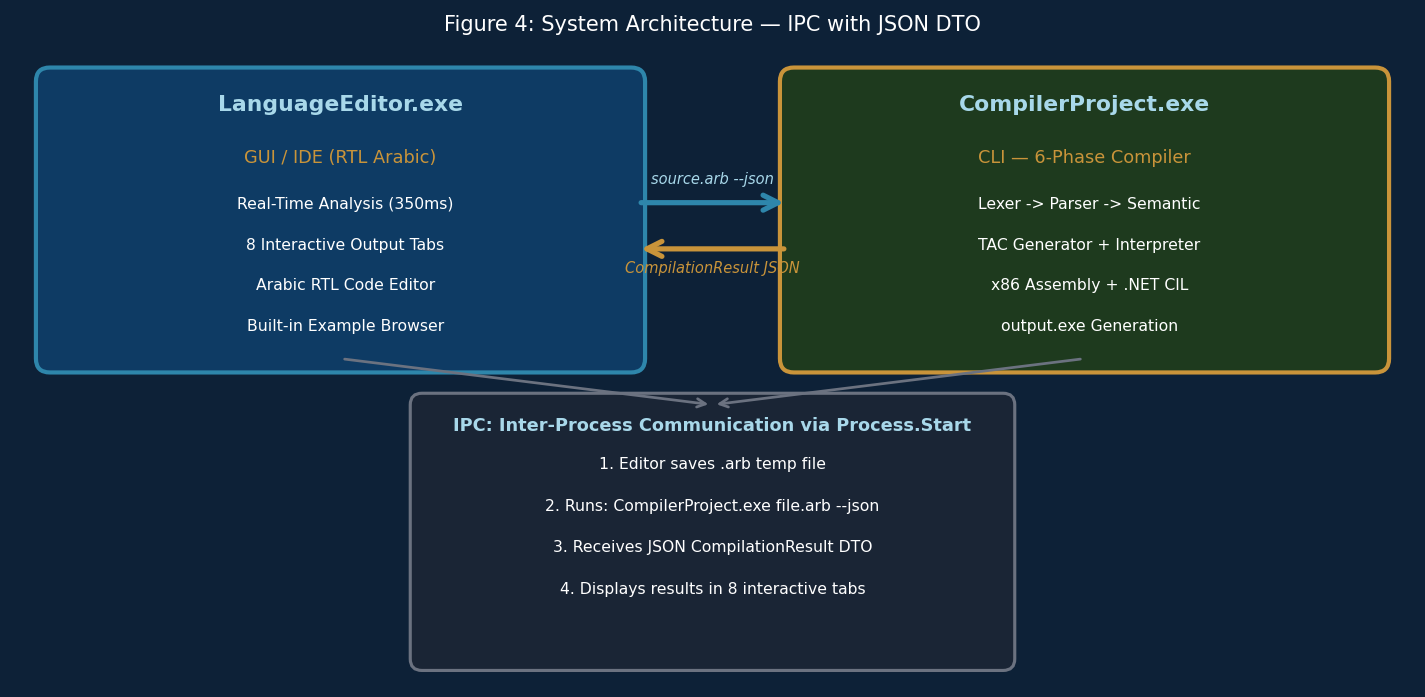
\includegraphics[width=0.92\textwidth]{imgs/fig04_arch.png}
    \caption{معمارية النظام المتكاملة والفصل التام بين محرر اللغة ومترجم C++ المستقل عبر IPC Pipes}
\end{figure}

\section{قواعد لغة البرمجة بصيغة EBNF الموسعة}
\begin{tcolorbox}[colback=BgLight,colframe=BorderGray,title={\small\arabicfont قواعد اللغة العربية بصيغة EBNF}]
\begin{lstlisting}
<برنامج>          ::= "برنامج" <معرف> "؛" <كتلة> "."
<كتلة>           ::= [<قسم_التصريحات>] "{" <قائمة_الجمل> "}"
<قسم_التصريحات>   ::= {<تصريح_ثابت> | <تصريح_متغير> | <تصريح_نوع>}
<تصريح_متغير>    ::= "متغير" <معرف> {"،" <معرف>} ":" <نوع_البيانات> "؛"
<تصريح_ثابت>     ::= "ثابت" <معرف> "=" <قيمة_ثابتة> "؛"
<نوع_البيانات>    ::= "صحيح" | "حقيقي" | "منطقي" | "حرفي" | "خيط_رمزي"
<جملة_شرطية>     ::= "اذا" "(" <تعبير> ")" "فان" <جملة> ["والا" <جملة>]
<حلقة_كرر>       ::= "كرر" "(" <معرف> "=" <تعبير> "الى" <تعبير> ["اضف" <تعبير>] ")" <جملة>
<حلقة_طالما>     ::= "طالما" "(" <تعبير> ")" "استمر" <جملة>
<حلقة_اعد>       ::= "اعد" <جملة> "حتى" "(" <تعبير> ")" "؛"
<تعليمة_قراءة>   ::= ("اقرا" | "اقرأ" | "اقرء") ["("] <معرف> [")"] "؛"
<تعليمة_طباعة>   ::= "اطبع" "(" <تعبير> {"،" <تعبير>} ")" "؛"
\end{lstlisting}
\end{tcolorbox}

\begin{figure}[htbp]
    \centering
    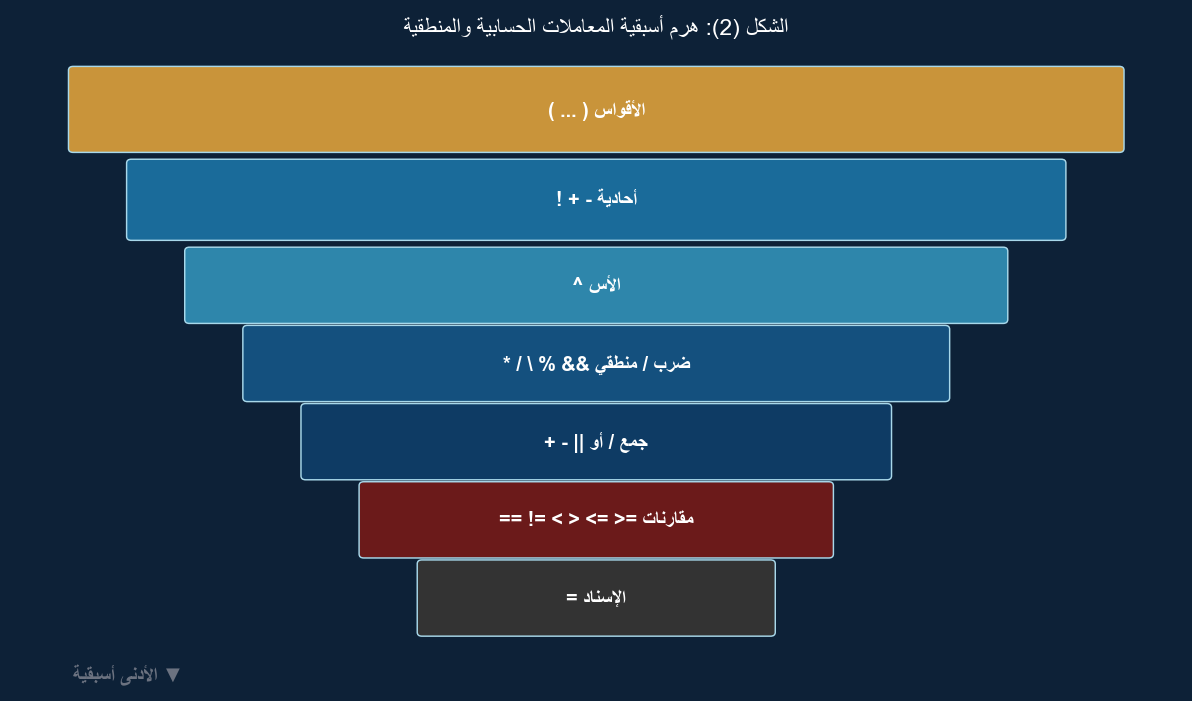
\includegraphics[width=0.85\textwidth]{imgs/fig08_ops.png}
    \caption{هرم أسبقية المعاملات الحسابية والمنطقية المعتمدة في المترجم}
\end{figure}

\begin{figure}[htbp]
    \centering
    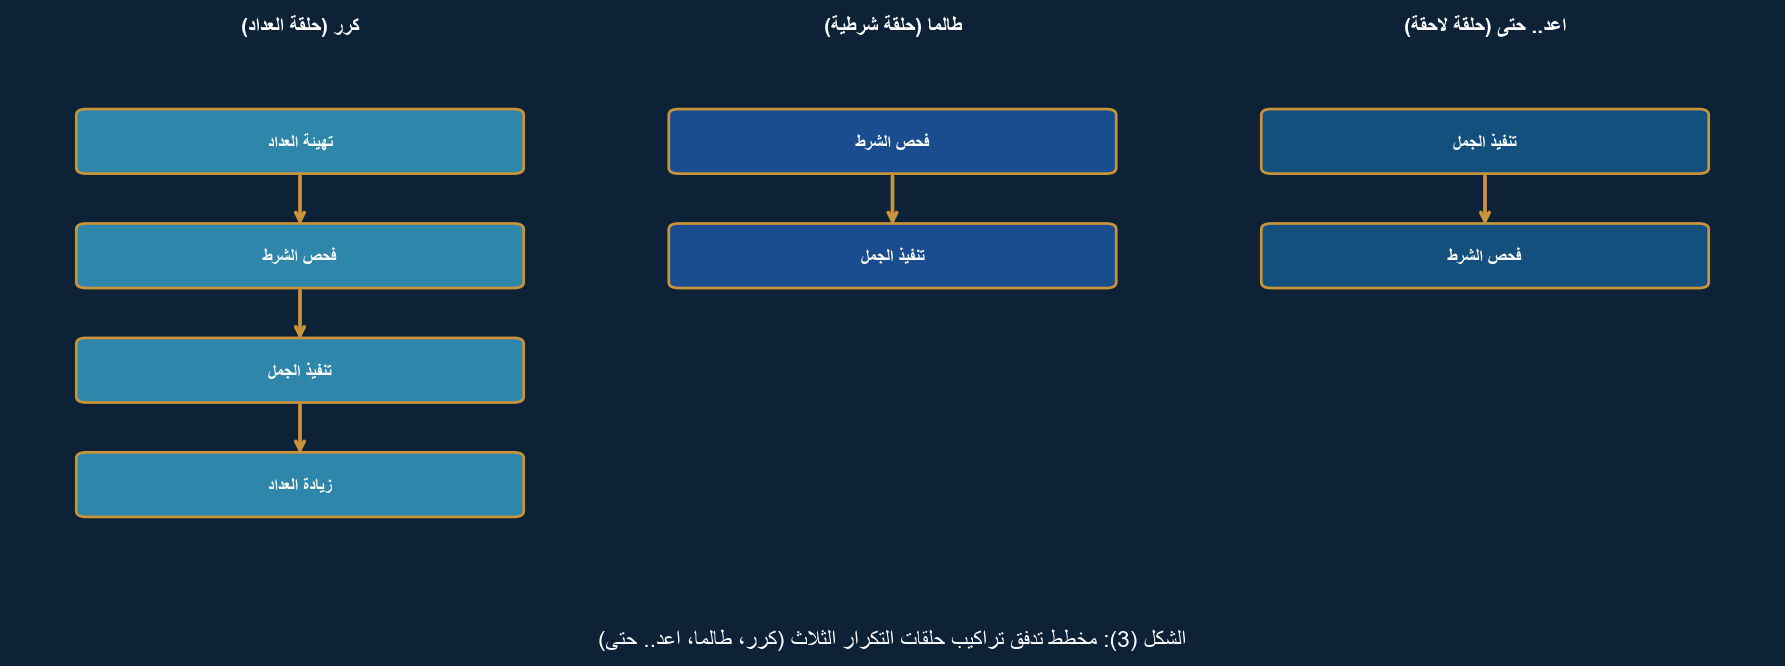
\includegraphics[width=0.85\textwidth]{imgs/fig06_loops.png}
    \caption{مخطط تدفق تراكيب حلقات التكرار الثلاث (كرر، طالما، اعد.. حتى)}
\end{figure}

% ═══════════════════════════════════════════════════════════════════════════════
% الفصل الخامس: حزمة الأمثلة الاختبارية العشرة
% ═════════════════════════════════════════════════════════════════════════
\chapter{حزمة الأمثلة الاختبارية العشرة المعتمدة}

تم إعداد واختبار 10 برامج شاملة ومتنوعة تثبت صحة عمل المترجم والمحرر عبر كافة التراكيب اللغوية:

\section{المثال 1: تعريف المتغيرات والعمليات الحسابية الأساسية}
\begin{tcolorbox}[colback=BgLight,colframe=BorderGray]
\begin{lstlisting}
برنامج حساب_المستطيل ؛
متغير
    الطول , العرض , المساحة : صحيح ؛
{
    الطول = 15 ؛
    العرض = 10 ؛
    المساحة = الطول * العرض ؛
    اطبع ( "مساحة المستطيل تساوي:" , المساحة ) ؛
} .
\end{lstlisting}
\end{tcolorbox}
\textbf{الهدف:} إثبات صحة التصريح عن المتغيرات وإجراء عمليات الضرب والإسناد والطباعة.\\
\textbf{المخرجات المتوقعة:} \texttt{مساحة المستطيل تساوي: 150}

\section{المثال 2: العمليات الحسابية المعقدة وأسبقية المعاملات}
\begin{tcolorbox}[colback=BgLight,colframe=BorderGray]
\begin{lstlisting}
برنامج اسبقية_العمليات ؛
متغير
    س , ص , ع , نتيجة : صحيح ؛
{
    س = 20 ؛ ص = 4 ؛ ع = 2 ؛
    نتيجة = س + ص * ع - 10 / 2 ؛
    اطبع ( "النتيجة النهائية هي:" , نتيجة ) ؛
} .
\end{lstlisting}
\end{tcolorbox}
\textbf{الهدف:} إثبات تطبيق أسبقية الضرب والقسمة قبل الجمع والطرح بدقة.\\
\textbf{المخرجات المتوقعة:} \texttt{النتيجة النهائية هي: 23}

\section{المثال 3: الجمل الشرطية البسيطة والمركبة (اذا / فان / والا)}
\begin{tcolorbox}[colback=BgLight,colframe=BorderGray]
\begin{lstlisting}
برنامج فحص_الدرجات ؛
متغير
    الدرجة : صحيح ؛
{
    الدرجة = 85 ؛
    اذا ( الدرجة >= 90 ) فان {
        اطبع ( "التقدير: ممتاز" ) ؛
    } والا {
        اذا ( الدرجة >= 75 ) فان {
            اطبع ( "التقدير: جيد جدا" ) ؛
        } والا {
            اطبع ( "التقدير: مقبول" ) ؛
        } ؛
    } ؛
} .
\end{lstlisting}
\end{tcolorbox}
\textbf{الهدف:} إثبات إعراب الشروط المتداخلة وتوليد قفزات TAC.\\
\textbf{المخرجات المتوقعة:} \texttt{التقدير: جيد جدا}

\section{المثال 4: حلقة العداد التراكمية المحددة (كرر)}
\begin{tcolorbox}[colback=BgLight,colframe=BorderGray]
\begin{lstlisting}
برنامج مجموع_الاعداد ؛
متغير
    العداد , المجموع : صحيح ؛
{
    المجموع = 0 ؛
    كرر العداد من 1 الى 10 اضف 1 {
        المجموع = المجموع + العداد ؛
    } ؛
    اطبع ( "مجموع الأرقام من 1 إلى 10 هو:" , المجموع ) ؛
} .
\end{lstlisting}
\end{tcolorbox}
\textbf{الهدف:} إثبات بناء عقد حلقة كرر وتوليد قفزات الزيادة التلقائية للعداد.\\
\textbf{المخرجات المتوقعة:} \texttt{مجموع الأرقام من 1 إلى 10 هو: 55}

\section{المثال 5: حلقة الدوران بالشرط المسبق (طالما ... استمر)}
\begin{tcolorbox}[colback=BgLight,colframe=BorderGray]
\begin{lstlisting}
برنامج حساب_القوى ؛
متغير
    الاساس , العداد , الناتج : صحيح ؛
{
    الاساس = 2 ؛ العداد = 1 ؛ الناتج = 1 ؛
    طالما ( العداد <= 5 ) استمر {
        الناتج = الناتج * الاساس ؛
        العداد = العداد + 1 ؛
    } ؛
    اطبع ( "2 أس 5 يساوي:" , الناتج ) ؛
} .
\end{lstlisting}
\end{tcolorbox}
\textbf{الهدف:} إثبات فحص الشرط المسبق وتكرار الكتلة البرمجية.\\
\textbf{المخرجات المتوقعة:} \texttt{2 أس 5 يساوي: 32}

\section{المثال 6: حلقة الدوران بالتحقق اللاحق (اعد ... حتى)}
\begin{tcolorbox}[colback=BgLight,colframe=BorderGray]
\begin{lstlisting}
برنامج اختبار_اعد_حتى ؛
متغير
    قيمة_س : صحيح ؛
{
    قيمة_س = 1 ؛
    اعد {
        قيمة_س = قيمة_س * 2 ؛
    } حتى ( قيمة_س >= 16 ) ؛
    اطبع ( "القيمة بعد انتهاء الحلقة هي:" , قيمة_س ) ؛
} .
\end{lstlisting}
\end{tcolorbox}
\textbf{الهدف:} إثبات تنفيذ جسم الحلقة مرة واحدة على الأقل وفحص شرط الخروج اللاحق.\\
\textbf{المخرجات المتوقعة:} \texttt{القيمة بعد انتهاء الحلقة هي: 16}

\section{المثال 7: تعليمة القراءة من المستخدم (اقرا) والطباعة}
\begin{tcolorbox}[colback=BgLight,colframe=BorderGray]
\begin{lstlisting}
برنامج مضاعفة_المدخلات ؛
متغير
    العدد_المدخل , الناتج : صحيح ؛
{
    اطبع ( "ادخل عددا ليتم مضاعفته:" ) ؛
    اقرا ( العدد_المدخل ) ؛
    الناتج = العدد_المدخل * 2 ؛
    اطبع ( "ضعف العدد المدخل هو:" , الناتج ) ؛
} .
\end{lstlisting}
\end{tcolorbox}
\textbf{الهدف:} إثبات معالجة مدخلات المستخدم من حقل الإدخال عبر Stdin بدون تعليق المترجم.\\
\textbf{المدخل التجريبي:} 25 $\rightarrow$ \textbf{المخرجات المتوقعة:} \texttt{ضعف العدد المدخل هو: 50}

\section{المثال 8: البرنامج الشامل لكافة القواعد والتراكيب}
\begin{tcolorbox}[colback=BgLight,colframe=BorderGray]
\begin{lstlisting}
برنامج النظام_الشامل ؛
ثابت
    النسبة_المئوية = 100 ؛
متغير
    الرقم , المجموع , الضرب : صحيح ؛
{
    الرقم = 5 ؛ المجموع = 0 ؛ الضرب = 1 ؛
    اذا ( الرقم > 0 ) فان {
        طالما ( الرقم > 0 ) استمر {
            المجموع = المجموع + الرقم ؛
            الضرب = الضرب * الرقم ؛
            الرقم = الرقم - 1 ؛
        } ؛
    } ؛
    اطبع ( "المجموع التراكمي:" , المجموع ) ؛
    اطبع ( "المضروب الرياضي:" , الضرب ) ؛
} .
\end{lstlisting}
\end{tcolorbox}
\textbf{الهدف:} إثبات تكامل الثوابت والمتغيرات والشروط وحلقات التكرار في برنامج واحد.\\
\textbf{المخرجات المتوقعة:} \texttt{المجموع التراكمي: 15} ثم \texttt{المضروب الرياضي: 120}

\section{المثال 9: كشف الأخطاء النحوية (Syntax Errors Negative Test)}
\begin{tcolorbox}[colback=BgLight,colframe=BorderGray]
\begin{lstlisting}
برنامج خطأ_نحوي_تجريبي ؛
متغير
    س , ص : صحيح ؛
{
    س = 10
    ص = س + * 5 ؛
    اذا ( س > 5 ) {
        اطبع ( س ) ؛
    } ؛
} .
\end{lstlisting}
\end{tcolorbox}
\textbf{الهدف:} اختبار متانة المحلل النحوي في كشف نسيان الفاصلة المنقوطة وتعاقب المعاملات ومواصلة الإعراب (Panic Mode).

\section{المثال 10: كشف الأخطاء الدلالية وحماية الثوابت (Semantic Errors Negative Test)}
\begin{tcolorbox}[colback=BgLight,colframe=BorderGray]
\begin{lstlisting}
برنامج خطأ_دلالي_تجريبي ؛
ثابت
    الحد_الثابت = 50 ؛
متغير
    س : صحيح ؛
{
    س = 20 ؛
    الحد_الثابت = 100 ؛
    غير_معرف = س + 5 ؛
    اقرا ( الحد_الثابت ) ؛
} .
\end{lstlisting}
\end{tcolorbox}
\textbf{الهدف:} اختبار المحلل الدلالي في منع تعديل الثوابت ومنع القراءة إليها وكشف المتغيرات غير المصرح بها بدقة متناهية.

% ═══════════════════════════════════════════════════════════════════════════════
% الفصل السادس: التوثيق التطبيقي المصور
% ═════════════════════════════════════════════════════════════════════════
\chapter{التوثيق التطبيقي المصور ومخرجات تنفيذ المشروع}

\begin{figure}[htbp]
    \centering
    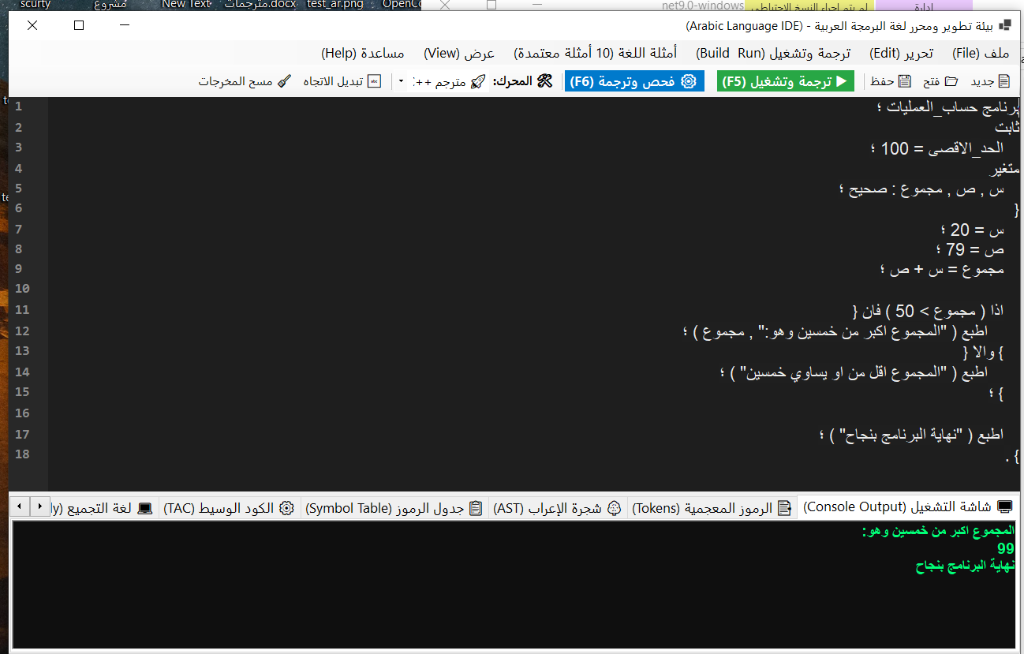
\includegraphics[width=0.92\textwidth]{imgs/real_screen01_ide_console.png}
    \caption{واجهة المحرر التفاعلية الرئيسية وتشغيل مخرجات الكونسول مع حقل إدخال تعليمة اقرا وزر التحديث}
\end{figure}

\begin{figure}[htbp]
    \centering
    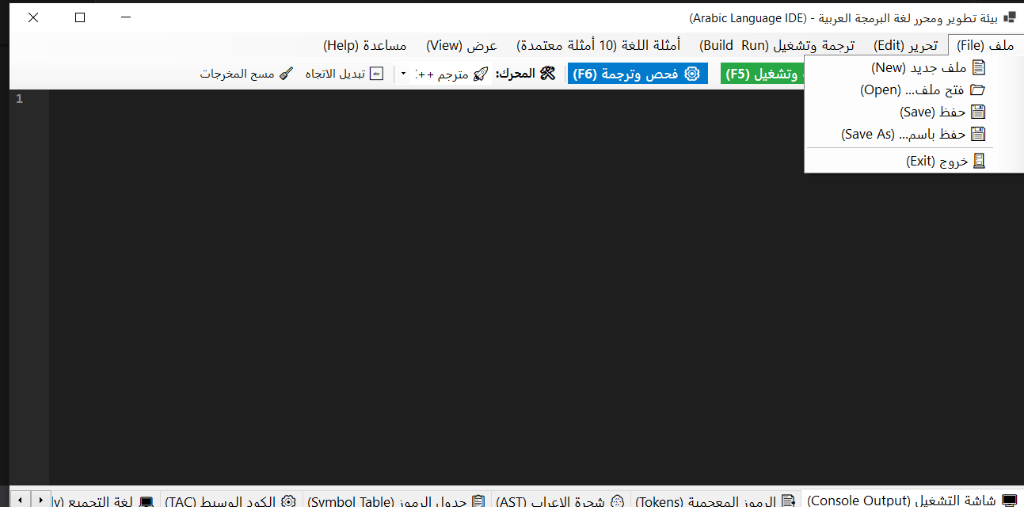
\includegraphics[width=0.92\textwidth]{imgs/real_screen02_file_menu.png}
    \caption{القوائم الرئيسية وإدارة الملفات والمشاريع (جديد، فتح، حفظ، حفظ باسم، خروج)}
\end{figure}

\begin{figure}[htbp]
    \centering
    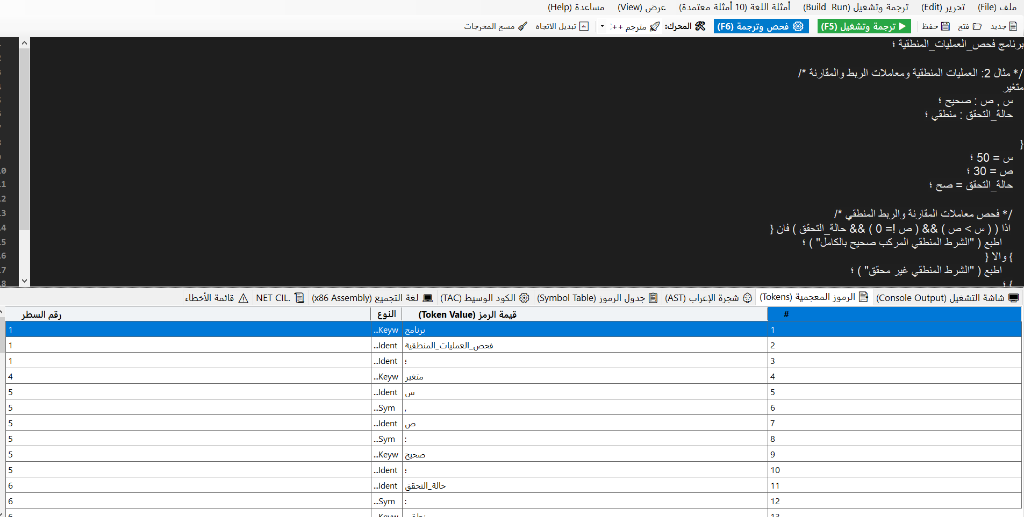
\includegraphics[width=0.92\textwidth]{imgs/real_screen03_tokens_grid.png}
    \caption{جدول استخراج الرموز المعجمية (Tokens DataGridView) في مترجم C++}
\end{figure}

\begin{figure}[htbp]
    \centering
    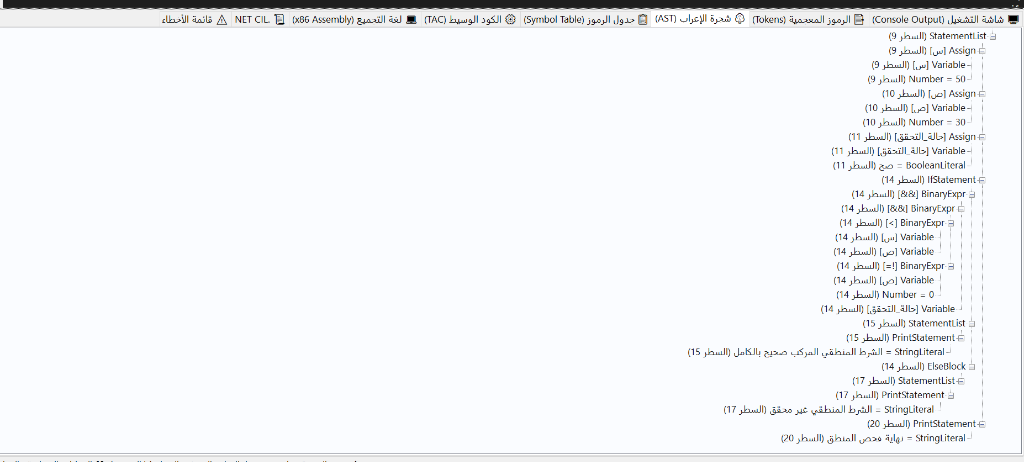
\includegraphics[width=0.92\textwidth]{imgs/real_screen04_ast_tree.png}
    \caption{شجرة الإعراب والاشتقاق النحوي الهرمية التفاعلية (AST Parse Tree)}
\end{figure}

\begin{figure}[htbp]
    \centering
    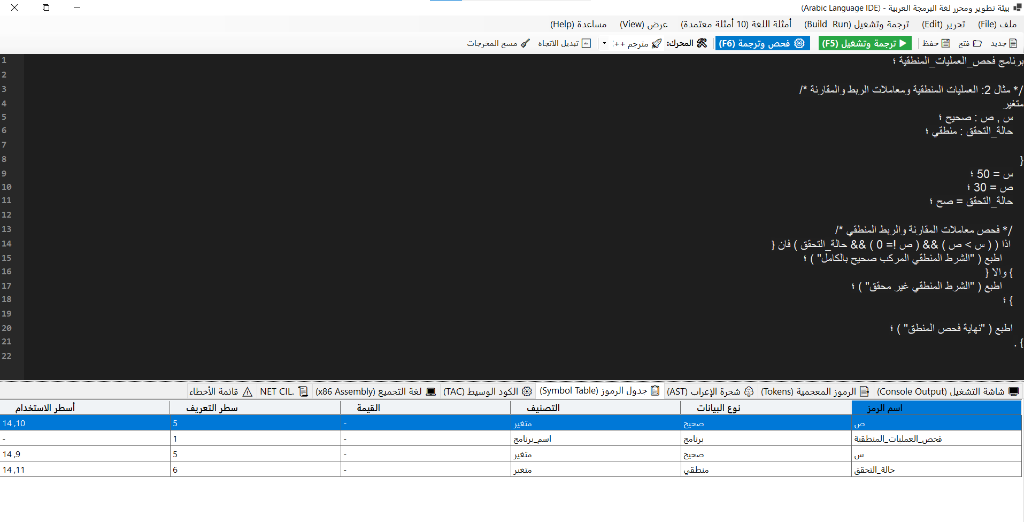
\includegraphics[width=0.92\textwidth]{imgs/real_screen05_symbol_table.png}
    \caption{جدول الرموز وإدارة النطاقات والمراجع وتتبع أسطر الاستخدام}
\end{figure}

\begin{figure}[htbp]
    \centering
    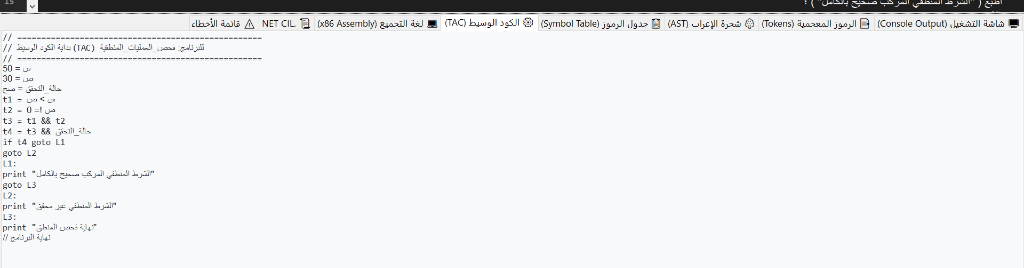
\includegraphics[width=0.92\textwidth]{imgs/real_screen06_tac_code.png}
    \caption{الشفرة الوسيطة ثلاثية العناوين (Three-Address Code -- TAC) المولدة من مترجم C++}
\end{figure}

\begin{figure}[htbp]
    \centering
    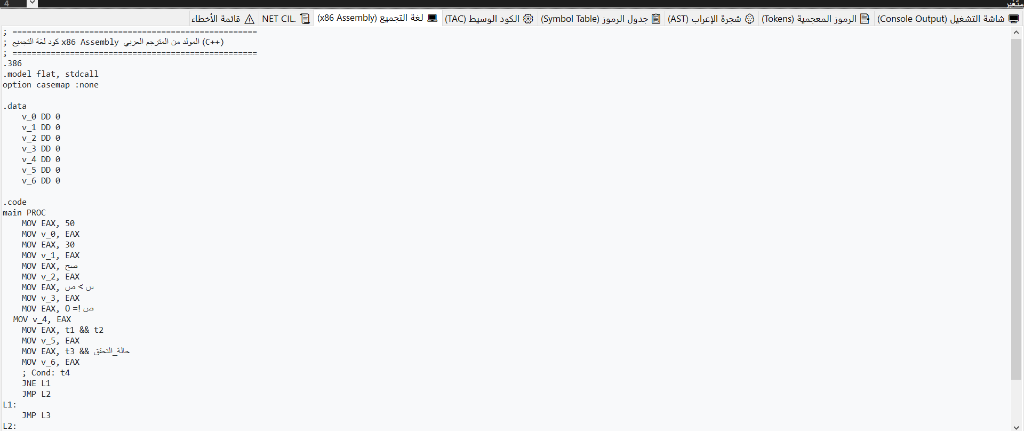
\includegraphics[width=0.92\textwidth]{imgs/real_screen07_assembly.png}
    \caption{شفرة لغة التجميع x86 بنمط MASM المولدة ذاتيا من المترجم}
\end{figure}

\begin{figure}[htbp]
    \centering
    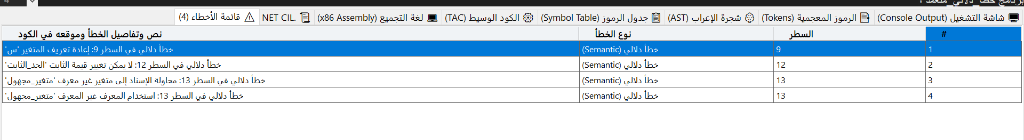
\includegraphics[width=0.92\textwidth]{imgs/real_screen08_error_list.png}
    \caption{قائمة تشخيص الأخطاء التفاعلية والتحقق الدلالي والانتقال الفوري لموضع الخطأ}
\end{figure}

% ═══════════════════════════════════════════════════════════════════════════════
% الفصل السابع: شروط وملفات التسليم النهائي
% ═════════════════════════════════════════════════════════════════════════
\chapter{شروط وملفات التسليم النهائي للمشروع}

وفقا للتعليمات الرسمية المعتمدة للمشروع، تم إعداد وحزم الملفات الثلاثة المطلوبة وتسميتها بكود المجموعة:
\begin{enumerate}
    \item \textbf{ملف التقرير الأكاديمي الشامل (\texttt{RPT-GXX.pdf}):} ملف بصيغة PDF معد وموثق وفق أعلى المعايير الأكاديمية ونظام APA 7th.
    \item \textbf{الملف التنفيذي المستقل للمشروع (\texttt{PREXE-GXX.exe}):} حزمة تشغيل مباشرة وتثبيت ذاتي تضم مترجم C++ المستقل ومحرر الأكواد معا.
    \item \textbf{ملف الأكواد المصدري المضغوط (\texttt{PRFL-GXX.rar}):} أرشيف مضغوط يضم كافة الأكواد المصدرية لمترجم C++ ومحرر C\# والأمثلة العشرة وملفات البناء المباشر.
\end{enumerate}

% ═══════════════════════════════════════════════════════════════════════════════
% المراجع والمصادر العلمية المعتمدة (APA 7th Edition)
% ═════════════════════════════════════════════════════════════════════════
\chapter*{المراجع والمصادر العلمية المعتمدة (APA 7th Edition)}
\addcontentsline{toc}{chapter}{المراجع والمصادر العلمية المعتمدة (APA 7th Edition)}

\begin{itemize}
    \item Aho, A. V., Lam, M. S., Sethi, R., \& Ullman, J. D. (2007). \textit{Compilers: Principles, techniques, and tools} (2nd ed.). Addison-Wesley.
    \item Al-Kahsah, K. M. (2025). \textit{Compiler construction course project specifications and Arabic grammar rules} (CS 351). Faculty of Computer Science and Information Technology, Ibb University.
    \item Al-Sharfi, A. (2026). \textit{Practical compiler construction and laboratory delivery guidelines}. Faculty of Computer Science and Information Technology, Ibb University.
    \item Cooper, K. D., \& Torczon, L. (2012). \textit{Engineering a compiler} (2nd ed.). Morgan Kaufmann.
    \item Grune, D., \& Jacobs, C. J. H. (2008). \textit{Parsing techniques: A practical guide} (2nd ed.). Springer.
    \item International Organization for Standardization. (2020). \textit{Programming languages --- C++} (ISO/IEC 14882:2020). ISO.
    \item Irvine, K. R. (2014). \textit{Assembly language for x86 processors} (7th ed.). Pearson.
    \item Louden, K. C. (1997). \textit{Compiler construction: Principles and practice}. PWS Publishing Company.
    \item Microsoft Corporation. (2024). \textit{C\# language reference, version 13.0 (.NET 9.0)}. Microsoft Learn. \url{https://learn.microsoft.com/en-us/dotnet/csharp/}
    \item Scott, M. L. (2015). \textit{Programming language pragmatics} (4th ed.). Morgan Kaufmann.
    \item Unicode Consortium. (2023). \textit{The Unicode standard, version 15.1.0}. \url{https://www.unicode.org/}
\end{itemize}

\end{document}
